\documentclass[a4paper]{article}

\usepackage[T1]{fontenc}
\usepackage[utf8]{inputenc}
\usepackage{lmodern}
\usepackage{mathtools}
\usepackage{palatino}
\usepackage{amssymb}
\usepackage{amsthm}
\usepackage{graphicx}
\usepackage{subcaption}
\usepackage{booktabs}
\usepackage{tabulary}
\usepackage{rotating}
\usepackage[margin=2cm]{geometry}
\usepackage{listings}
\usepackage[ruled,vlined]{algorithm2e}
\usepackage{hyperref}
\usepackage{todonotes}
\usepackage[round,sort&compress]{natbib}
\usepackage[acronym,smallcaps,nowarn,section,nogroupskip,nonumberlist]{glossaries}

% Bibliography
\bibliographystyle{unsrtnat}

% Abbreviations
\glsdisablehyper{}
\newacronym{VAE}{vae}{variational auto-encoder}

% Skip line instead of indent
\usepackage[parfill]{parskip}

\newcommand{\given}{\lvert}
\DeclareMathOperator{\E}{\mathbb{E}}

\title{Agent Models}
% \author{Author 1, Author 2}
% \date{\today}

\begin{document}
\maketitle

\section{Talking Pedestrians}
There are two pedestrians on the pavement, facing each other and talking.
One of them suddenly decides to cross the road and starts turning his body to do so.
An approaching car should reason about the intentions of this person and predict their future path and depending on it make a decision to continue going or stop to wait for the person to cross.
\begin{figure}[htb]
    \centering
    \begin{subfigure}[t]{0.3\textwidth}
        \centering
        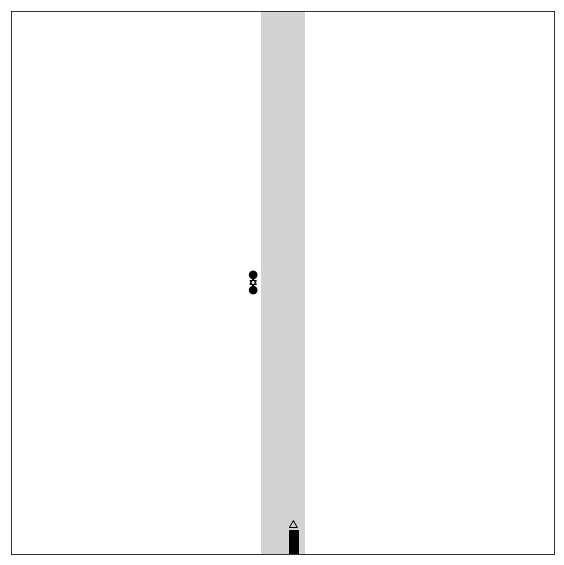
\includegraphics[width=\textwidth]{figures/talking_pedestrians_1.png}
        \caption{Pedestrians are talking.}
    \end{subfigure}
    ~ 
    \begin{subfigure}[t]{0.3\textwidth}
        \centering
        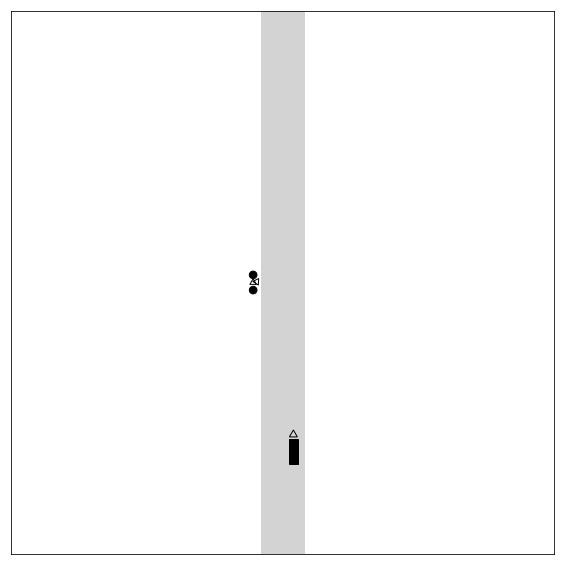
\includegraphics[width=\textwidth]{figures/talking_pedestrians_2.png}
        \caption{Pedestrian decides to cross the road and turns towards the road.}
    \end{subfigure}
    ~
    \begin{subfigure}[t]{0.3\textwidth}
        \centering
        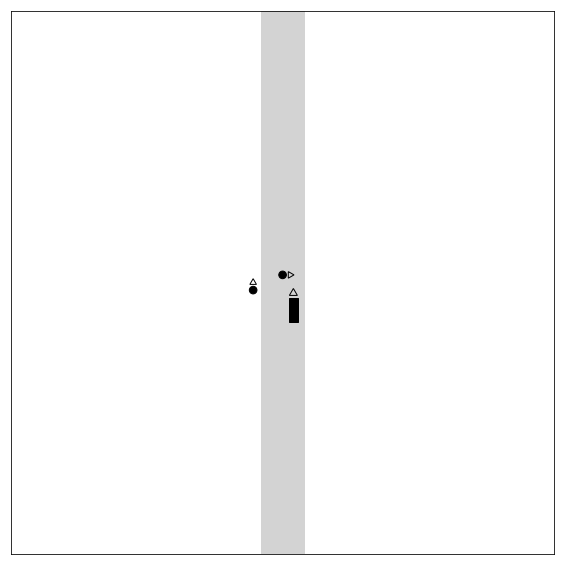
\includegraphics[width=\textwidth]{figures/talking_pedestrians_3.png}
        \caption{Pedestrian crosses the road. The car waits.}
    \end{subfigure}
    \caption{Talking Pedestrians.}
\end{figure}

\paragraph{Pedestrian Model.}
For simplicity, we will only perform inference on one pedestrian.
Let $i_t, p_t, a_t$ be the pedestrian's intention, position and angle at time $t$, and let $o_t := (o_t^p, o_t^a)$ be the observation of that pedestrian's position and angle at time $t$. The graphical of this model is in Figure~\ref{fig:talking_pedestrians_4}.
\begin{figure}[htb]
    \centering
    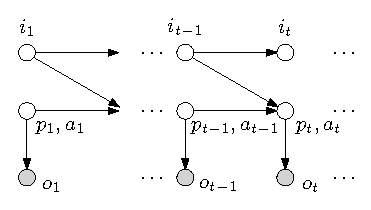
\includegraphics{figures/talking_pedestrians_4}
    \caption{Graphical model for the pedestrian.}
    \label{fig:talking_pedestrians_4}
\end{figure}

The probabilistic model is as follows:
\begin{align}
    p(i_1) &= \mathrm{Uniform}(i_1 \given \mathcal I) \\
    p(i_t \given i_{t - 1}) &=
        \begin{cases}
            1 - \epsilon & \text{if } i_t = i_{t - 1} \\
            \frac{\epsilon}{|\mathcal I| - 1} & \text{otherwise}
        \end{cases} \\
    p(p_1, a_1) &= \delta_{(o_1^p, o_1^a)}(p_1, a_1) \\
    p(p_t, a_t \given p_{t - 1}, a_{t - 1}, i_{t - 1}) &= \delta_{\pi(p_{t - 1}, a_{t - 1}, i_{t - 1})}(p_t, a_t) \\
    p(o_t \given p_t, a_t) &= \mathrm{Normal}(o_t^p \given p_t, \Sigma_p) \cdot \mathrm{Normal}(o_t^a \given a_t, \sigma_a^2), \label{eq:sensor}
\end{align}
$\mathcal I = \{\text{``cross''}, \text{``talk''}, \text{``idle''}\}$ are the possible intentions,
$\epsilon$ is the probability of switching intentions,
$\pi$ is a pedestrian policy which we will describe later,
$\delta_z$ is a delta mass at $z$,
and $\Sigma_p$ and $\sigma_a^2$ are the position and angle sensor (co)variances.

\paragraph{Pedestrian's Policy.}
The pedestrian policy $\pi$ maps from $p_t, a_t, i_t$ to $p_{t + 1}, a_{t + 1}$.
It is notationally cleaner to describe in words.
If $i_t = \text{``idle''}$, $\pi(p_t, a_t, i_t) = (p_t, a_t)$.
If $i_t = \text{``talk''}$, the pedestrian rotates and moves to the left side of the road where they then rotate and talk to their friend.
If $i_t = \text{``cross''}$, the pedestrian rotates and moves to the right side of the road where they stay.
Note that this function branches according to $i_t$.

\paragraph{Car's Policy.}
The car's policy is a function $\rho(j_t, c_t, o_{1:t})$ which takes in the car's intention $j_t$ and position $c_t$ and the observations $o_{1:t}$ of the pedestrian; it returns the next car position $c_{t + 1}$.

The car's intention is an element of $\mathcal J = \{\text{``go''}, \text{``go careful''}, \text{``wait''}, \text{``idle''}\}$.
If $j_t = \text{``idle''}$, $\rho(j_t, c_t, o_{1:t}) = c_t$.
If $j_t = \text{``go''}$, the car goes with an average speed to the end of the road.
If $j_t = \text{``wait''}$, the car goes with a slow speed to the start of the pedestrian crossing.

If $j_t = \text{``go careful''}$, things get interesting.
Let $L$ be the number of prediction steps.
First, we perform inference to obtain the prediction $p(p_{t + 1:t + L} \given o_{1:t})$ under the pedestrian model.
Second, we predict the car positions $c_{t + 1:t + L}$ if it were to use $j_{\tau} = \text{``go''}$ for $\tau = t + 1, \dotsc, t + L$.
Third, we define a risk function $R(p_{\tau}, c_{\tau})$ to be an indicator for both $p_{\tau}, c_{\tau}$ being on the pedestrian crossing (with some safety margin).
We arrive at the maximum expected risk:
\begin{align}
    r = \max_{\tau \in \{t + 1, \dotsc, t + L\}} \E_{p(p_{t + 1:t + L} \given o_{1:t})}\left[R(p_\tau, c_{\tau})\right]. \label{eq:risk}
\end{align}
If this quantity is larger than some safety tolerance $r_{\text{safe}}$, $\rho(j_t, c_t, o_{1:t}) = \rho(\text{``wait''}, c_t, o_{1:t})$, otherwise $\rho(j_t, c_t, o_{1:t}) = \rho(\text{``go''}, c_t, o_{1:t})$:
\begin{align}
    \rho(\text{``go careful''}, c_t, o_{1:t}) &=
    \begin{cases}
        \rho(\text{``wait''}, c_t, o_{1:t}) & \text{if } r > r_{\text{safe}} \\
        \rho(\text{``go''}, c_t, o_{1:t}) & \text{otherwise}.
    \end{cases}
\end{align}

Note that due to the uncertainty of the position and angle sensor (encoded in \eqref{eq:sensor}), there is an uncertainty about the person's intention and hence future position, over which we average over in \eqref{eq:risk}.

\section{Two Cars}
There are three agents: a car that we control (black), another car on the road (gray), and a pedestrian who is visible to the gray car, but not visible to our black car due to a building standing in a way.
Even though our car doesn't see the pedestrian, if it sees that the gray car is slowing down, it should infer that there indeed is a pedestrian behind the building and slows down to stop for the invisible pedestrian to cross.
This is illustrated in Figure~\ref{fig:talking_pedestrians_6}.
\begin{figure}[htb]
    \centering
    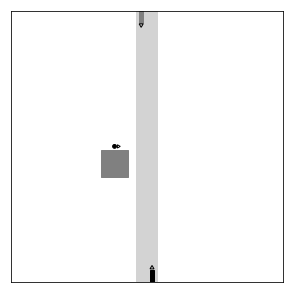
\includegraphics[width=0.3\textwidth]{figures/talking_pedestrians_6.png}
    \caption{Two cars and one pedestrian. Our black car doesn't see the pedestrian but the gray car does.}
    \label{fig:talking_pedestrians_6}
\end{figure}

\paragraph{Black Car's Model of the Pedestrian and the Gray Car.}
\begin{figure}[htb]
    \centering
    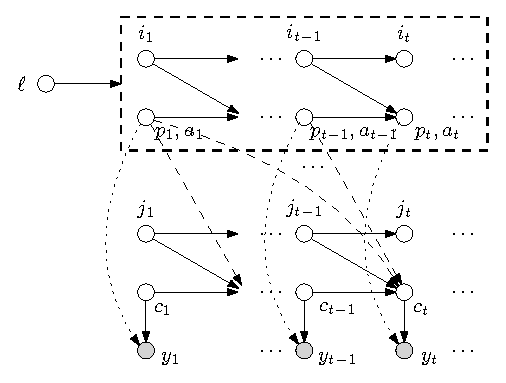
\includegraphics{figures/talking_pedestrians_5}
    \caption{Graphical model for the pedestrian and the gray car.}
    \label{fig:talking_pedestrians_5}
\end{figure}

The probabilistic model that the black car uses is shown in Figure~\ref{fig:talking_pedestrians_5}.

First, we have the gray car's intentions $j_t$ where the prior and the transition are:
\begin{align}
    p(j_1) &= \mathrm{Uniform}(\mathcal J) \\
    p(j_t \given j_{t - 1}) &= 
    \begin{cases}
        1 - \epsilon & \text{if } j_t = j_{t - 1} \\
        \frac{\epsilon}{|\mathcal J| - 1} & \text{otherwise},
    \end{cases}
\end{align}
where $\mathcal J = \{\text{``go''}, \text{``go careful''}, \text{``wait''}, \text{``idle''}\}$ like before.

The prior for $c_1$ is as follows:
\begin{align}
    p(c_1) &= \delta_{y_1^c}(c_1).
\end{align}

Next, we have the latent variable $\ell$ which indicates whether the person exists or not. We place a uniform prior on the person's existence:
\begin{align}
    p(\ell) &= \mathrm{Bernoulli}(0.5).
\end{align}
If the person exists ($\ell = 1$), the random variables $i_t, p_t, a_t$ in the thick dashed box exist and the transition is as follows:
\begin{align}
    p(c_t \given c_{t - 1}, j_{t - 1}, p_{1:t - 1}, a_{1:t - 1}) = \delta_{\rho\left(j_{t - 1}, c_{t - 1}, ((p_\tau, a_\tau))_{\tau = 1}^{t - 1}\right)}(c_t).
\end{align}
If the person doesn't exist ($\ell = 0$), the random variables $i_t, p_t, a_t$ in the thick dashed box don't exist and the transition is as follows:
\begin{align}
    p(c_t \given c_{t - 1}, j_{t - 1}) = \delta_{\rho'(c_{t - 1}, j_{t - 1})}(c_t),
\end{align}
where $\rho'(c, \text{``go careful''}) = \rho'(c, \text{``go''}) = \rho(c, \text{``go''}, o_{1:t})$ and $\rho'(c, \text{``wait''}) = \rho(c, \text{``wait''}, o_{1:t})$ and $\rho'(c, \text{``idle''}) = c$.

Finally, we have the likelihood for the observation $y_t = (y_t^c, y_t^p, y_t^a)$ or $y_t = y_t^c$ depending on whether our black car sees the pedestrian or not.
If $y_t = (y_t^c, y_t^p, y_t^a)$, the likelihood is as follows:
\begin{align}
    p(y_t \given c_t) &= \mathrm{Normal}(y_t^c \given c_t, \Sigma_c) \cdot \mathrm{Normal}(y_t^p \given p_t, \Sigma_p) \cdot \mathrm{Normal}(y_t^a \given a_t, \sigma_a^2).
\end{align}
If $y_t = y_t^c$, the likelihood is:
\begin{align}
    p(y_t \given c_t) &= \mathrm{Normal}(y_t^c \given c_t, \Sigma_c).
\end{align}

\paragraph{Black Car's Policy.}
The black car's policy is a function $\xi(k_t, d_t, y_{1:t})$ which takes in the black car's intention $k_t$, and position $d_t$, and the observations of the world $y_{1:t}$.

Similarly as before, if $k_t = \text{``idle''}$, $\xi(k_t, d_t, y_{1:t}) = d_t$.
If $k_t = \text{``go''}$, the car goes with an average speed to the other side of the road.
If $k_t = \text{``wait''}$, the car goes with a slow speed to the start of the pedestrian crossing.

If $k_t = \text{``go careful''}$, the black car's model is used to obtain the prediction of the person's position from $t + 1$ to $t + L$, $p(p_{t + 1:t + L} \given y_{1:t})$,  where $L$ is the number of prediction steps.
This prediction, together with the forward simulation of the black car assuming the $\text{``go''}$ intention throughout, $d_{t + 1:t + L}$, is used to evaluate the maximum expected risk for the black car:
\begin{align}
    s = \max_{\tau \in \{t + 1, \dotsc, t + L\}} \E_{p(p_{t + 1:t + L} \given y_{1:t})}[R(p_\tau, d_\tau)],
\end{align}
where the risk function $R$ is like before but evaluates to $0$ if the pedestrian doesn't exist.

Like before, 
\begin{align}
    \xi(\text{``go careful''}, d_t, o_{1:t}) &=
    \begin{cases}
        \xi(\text{``wait''}, d_t, o_{1:t}) & \text{if } s > r_{\text{safe}} \\
        \xi(\text{``go''}, d_t, o_{1:t}) & \text{otherwise}.
    \end{cases}
\end{align}

\section{Nested Inference}
Note that in the ``Two Car'' scenario, in order for the black car to make a decision, it must evaluate a function that is an expectation under the posterior predictive of of the black car's model of the pedestrian and the gray car, $p(p_{t + 1:t + L} \given y_{1:t})$.
However, a forward simulation under this model relies on evaluating the gray car's policy, $\rho$, which internally performs inference in the gray car's model of the pedestrian (in Figure~\ref{fig:talking_pedestrians_4}).

Let $\gamma_1(x_1)$ be an unnormalized density with the normalizing constant $Z_1$ and the normalized density $\pi_1(x_1) = \gamma_1(x_1) / Z_1$. We would like to evaluate $\E_{\pi_1(x_1)}[f_1(x_1)]$.
However, even evaluating $\gamma_1(x_1)$ requires evaluating $\E_{\pi_2(x_2)}[f_2(x_2)]$ where $\pi_2(x_2)$ is a normalized density with the normalizing constant $Z_2$ and the unnormalized version $\gamma_2(x_2) = Z_2 \pi_2(x_2)$.

\paragraph{Example.}{Let $\gamma_i(x_i) = p_i(y_i \given x_i) p_i(x_i)$, $\pi_i(x_i) = p_i(x_i \given y_i)$, $Z_i = p_i(y_i)$ and $f_i(x_i) = x_i^2$ for $i = 1, 2$, where
\begin{align}
    p_1(x_1) &= \mathrm{Normal}(x_1 \given \E_{p_2(x_2 \given y_2)}[f_2(x_2)], s_1^2), &
    p_1(y_1 \given x_1) &= \mathrm{Normal}(y_1 \given x_1, \sigma_1^2), \\
    p_2(x_2) &= \mathrm{Normal}(x_2 \given m_2, s_2^2), &
    p_2(y_2 \given x_2) &= \mathrm{Normal}(y_2 \given x_2, \sigma_2^2).
\end{align}
In this case, there is a closed form solution for $\E_{p_1(x_1 \given y_1)}[f_1(x_1)]$ given $y_1, y_2$.}

In general, how would we estimate $\E_{\pi_1(x_1)}[f_1(x_1)]$?
We could try nested importance sampling.
Will this result in a biased estimator?
Will it be efficient?
We could try to use inference compilation for the inner model $p_2(x_2, y_2)$.

These questions are somewhat answered by Tom's papers.

\begin{figure}[htb]
    \centering
    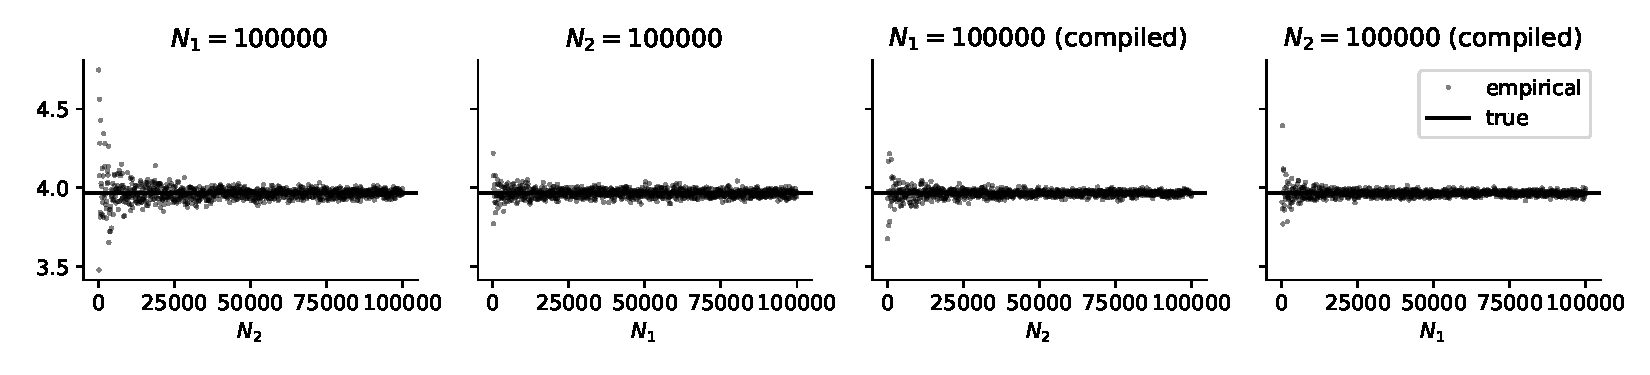
\includegraphics[width=0.8\textwidth]{figures/unbiasedness_together.pdf}
    \caption{Inner number of samples $N_2$ and outer number of samples $N_1$. $s_1 = \sigma_1 = s_2 = \sigma_2 = 1$, $m_2 = 0$, and $y_1 = 1.9, y_2 = 2.3$.}
    \label{fig:unbiasedness_together}
\end{figure}

\section{Model Learning and Amortizing Inference in Open Universe Models with Stochastic Control Flow}

The ``Talking Pedestrians'' model demonstrates a need for fast repeated inference.
The ``Two Cars'' model demonstrates a need for fast repeated nested inference.
Both models require discrete latent variables and stochastic control flow: intention of agents are modeled by discrete latent variables and the policy functions which drive the transition functions contain control flow where the condition is the intention variable.
The ``Two Cars'' model also demonstrates a need for open universe models only expressible in higher-order probabilistic programming languages.

We would like to be able to also learn the model given a family of open universe models with discrete latent variables and stochastic control flow.
Let's use CDAE.

\bibliography{models}
\end{document}
